\documentclass[11pt,a4paper]{article}
\usepackage[top=3cm, bottom=2cm, left=2cm, right=2cm]{geometry}
\usepackage[utf8]{inputenc}
\usepackage{amsmath, amsfonts, amssymb}
\usepackage{siunitx}
\usepackage[brazil]{babel}
\usepackage{graphicx}
\usepackage[margin=10pt,font={small, it},labelfont=bf, textfont=it]{caption}
\usepackage[dvipsnames, svgnames]{xcolor}
\DeclareCaptionFont{MediumOrchid}{\color[svgnames]{MediumOrchid}}
\usepackage[pdftex]{hyperref}
\usepackage{natbib}
\bibliographystyle{plainnat}
\bibpunct{\textcolor{MediumOrchid}{\textbf{[}}}{\textcolor{MediumOrchid}{\textbf{]}}}{,}{s}{}{}
\usepackage{color}
\usepackage{footnote}
\usepackage{setspace}
\usepackage{booktabs}
\usepackage{multirow}
\usepackage{subfigure}
\usepackage{fancyhdr}
\usepackage{leading}
\usepackage{indentfirst}
\usepackage{wrapfig}
\usepackage{mdframed}
\usepackage{etoolbox}
\usepackage[version=4]{mhchem}
\usepackage{enumitem}
\usepackage{caption}
\usepackage{titlesec}
\usepackage{tcolorbox}
\usepackage{tikz}
\usepackage{LobsterTwo}
\usepackage[T1]{fontenc}
\usepackage{fontspec}
\usepackage{txfonts}
\usepackage[bottom]{footmisc}
\tcbuselibrary{skins,breakable}
\sisetup{output-decimal-marker={.}}

\makeatletter
\def\footnoterule{\kern-3pt\color{MediumOrchid}\hrule\@width0.6\textwidth height 0.8pt\kern2.6pt}
\makeatother

\renewcommand{\footnotelayout}{\itshape\color{MediumOrchid}}

\AtBeginEnvironment{equation}{\fontsize{13}{16}\selectfont}


\titleformat{\section}{\LobsterTwo\LARGE\color{CarnationPink}}{\thesection.}{1em}{}
\titleformat{\subsection}{\LobsterTwo\LARGE\color{CarnationPink}}{\thesubsection}{1em}{}
\titleformat{\subsubsection}{\LobsterTwo\large\color{MediumOrchid}}{\thesubsubsection}{1em}{}


\DeclareCaptionLabelFormat{figuras}{\textcolor{DarkTurquoise}{Figura \arabic{figure}}}
\captionsetup[figure]{labelformat=figuras}

\makeatletter
\renewcommand\tagform@[1]{\maketag@@@{\color{CarnationPink}(#1)}}
\makeatother

\renewcommand{\theequation}{Eq. \arabic{equation}}
\renewcommand{\thefigure}{Fig. \arabic{figure}}
\renewcommand{\thesection}{\textcolor{CarnationPink}{\arabic{section}}}

\setlist[itemize]{label=\textcolor{CarnationPink}{$\blacksquare$}}

\setlist[enumerate]{label=\textcolor{CarnationPink}{\arabic*.}, align=left, leftmargin=1.5cm}


\newcounter{exemplo}

\NewDocumentEnvironment{exemplo}{ O{} }{%
\allowbreak
\setlength{\parindent}{0pt}
  \begin{mdframed}[
  leftline=true,
  topline=false,
  rightline=false,
  bottomline=false,
  linewidth=2pt,
  linecolor=CarnationPink,
  frametitlerule=false,
  frametitlefont=\LobsterTwo\large\color{CarnationPink},
  frametitle={\color{CarnationPink}\LobsterTwo\large #1},
  ]
}{%
  \end{mdframed}
}

\setlength{\fboxsep}{5pt}
\setlength{\fboxrule}{1.5pt}
\usepackage{float}
\renewcommand{\thefootnote}{\alph{footnote}}
\usepackage{url}
\hypersetup{
	colorlinks=true,
	linkcolor=DarkTurquoise,
	filecolor=DarkTurquoise,      
	urlcolor=DarkTurquoise,
	citecolor=DarkTurquoise,
	pdftitle={Especialista em Física da Radioterapia}
}
\pagestyle{fancy}
\fancyhf{}
\renewcommand{\headrulewidth}{0pt}
\rfoot{Página \thepage}

\title{\LobsterTwo\Huge{Braquiterapia}}
\author{\LobsterTwo\Large{Implantes de Próstata LDR}\nocite{*}}
\date{\LobsterTwo\textit{Dalila Mendonça}}
\begin{document}
	\maketitle

\section{Introdução}

	A braquiterapia da próstata é uma das várias técnicas de tratamento disponíveis para pacientes com doença localizada. A braquiterapia da próstata é atualmente praticada usando duas técnicas diferentes:

	\begin{enumerate}[label=\textcolor{CarnationPink}{\roman*.}]
		\item Implante de semente de próstata (PSI) usando fontes de baixa taxa de dose (LDR); e
		\item Braquiterapia de alta taxa de dose (HDR).
	\end{enumerate}

	Como outras tecnologias em Radioterapia, o implante de semente de próstada passou por grandes mudanças tanto na implementação da tecnologia quanto nas recomendações clínicas baseadas no conhecimento de ensaios clínicos. Inicialmente, as sementes soltas de \ce{^{103}Pd} eram a única fonte de radiação disponível para o implante. Em 1999, o Instituto Nacional de Padrões e Tecnologia (NIST) mudou seu padrão de calibração, levando a um ajuste de 9\% na calibração da dose. 
	
	\ce{^{125}I}, \ce{^{131}Cs} e \ce{^{198}Au} expandiram as opções para escolha da fontes das instituições que realizam implante de semente de próstada. Melhores tecnologias de ultrassom e computacionais permitiram a mudança para o pré-planejamento baseado em imagens 3D ou planejamento diretamente na sala de cirurgia (RO). Os fornecedores desenvolveram agulhas pré-carregadas, configurações de sementes em forma de fios e tecnologia  ``stranding'' que podem ser usadas para montar fios na própria sala de cirurgia. Fornecedores terceirizados agora estão oferecendo ensaios independentes das sementes, o que levou a AAPM a mudar a recomendação para ensaios clínicos de sementes.

	Os critérios de seleção de pacientes e os regimes de tratamento para implante de semente de próstada estão em constante evolução à medida que mais dados clínicos se tornam disponíveis. O paciente que ira realizar implante de semente de próstada ``clássico'' como tratamento exclusivo tem doença de baixo grau, em estágio inicial. O implante de semente de próstada também é uma alternativa para pacientes de risco intermediário, seja como terapia exclusiva ou em combinação com outras terapias. O guideline do American College of Radiology (ACR)-American Society for Radiation Oncology (ASTRO) para a braquiterapia transperineal permanente do câncer de próstata sugere que ``cada instalação estabeleça e siga suas próprias diretrizes práticas. Os ensaios clínicos em andamento ajudarão a definir melhor as indicações do tratamento''. 

	As recomendações da American Brachytherapy Society (ABS) para braquiterapia transperineal permanente do câncer de próstata, publicadas em 1999, discutem com mais detalhes os critérios de seleção dos pacientes com base nos fundamentos clínicos extraídos de revisões da literatura e da extensa experiência clínica dos autores. Esse guideline foi atualizado em 2012. Em geral, os pacientes com doença de baixo risco, com boa expectativa de vida, com função urinária aceitável e com anatomia favorável são bons candidatos à braquiterapia de próstata como terapia exclusiva. Pacientes selecionados com doença de risco intermediário ou alto risco também podem ser candidatos à braquiterapia, especialmente como um boost em conjunto com a teleterapia.

	Várias sociedades desenvolveram recomendações sobre muitos aspectos do implante de semente de próstada. O ACR e a ASTRO colaboraram para publicar guidelines práticos destinados a toda a equipe de tratamento e guidelines técnicos de alto nível para físicos. A ABS possui uma série de recomendações dirigidas tanto a médicos quanto a físicos. O AAPM Task Group (TG)-64 sobre implante de semente de próstada, o AAPM TG-128, \textit{``Quality Assurance Tests for Prostate Brachytherapy Ultrasound Systems''} e white papers oferecem recomendações sobre dosimetria e garantia da qualidade (QA) para o  físico médico.

\section{Fontes}

\subsection*{Fontes LDR}

	O césio é o isótopo mais recente desenvolvido para implante de semente de próstada (\ref{fig:fontesBraquiProstata}). Devido à sua meia-vida muito curta, pode haver uma vantagem biológica na entrega mais rápida da dose, possivelmente com menores taxas de complicações a longo prazo. Esse raciocínio é semelhante aos argumentos que conduzem os ensaios clínicos para radioterapia estereotáxica da próstata (SBRT) e a HDR.

	\begin{figure}[h]
		\centering
		\fcolorbox{DarkTurquoise}{white}{%
			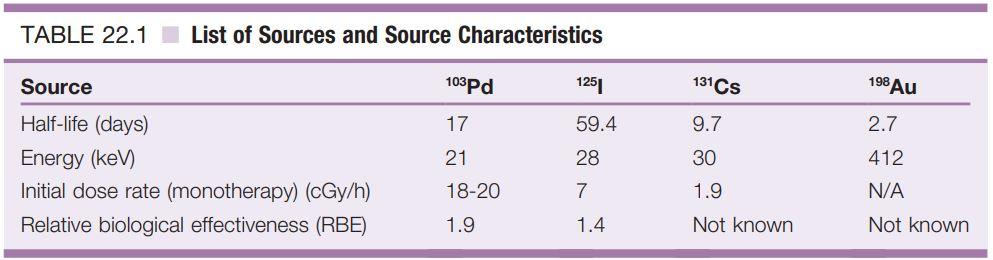
\includegraphics[width=0.8\textwidth]{Imagens/fontesBraquiProstata.JPG}
		}%
		\caption{Lista de fontes e características da fonte}
		\label{fig:fontesBraquiProstata}
	\end{figure}

	Embora alguns estudos tenham mostrado uma vantagem de um isótopo sobre outro em ensaios clínicos muito selecionados, outros estudos contradizem esses achados. Os estudos clínicos não mostraram nenhuma diferença estatisticamente significativa entre os isótopos com base no resultado ou na toxicidade do tratamento. O tempo para o desenvolvimento de toxicidade uretral e retal é menor para isótopos de meia-vida mais curta. Isótopos de menor energia fazem com que a dose entregue seja mais sensível ao espaçamento das sementes.

	O AAPM TG-43 em braquiterapia, \textit{``Dosimetry of Intersticial Brachytherapy Sources''}, especifica o cálculo da dose no tecido para os vários isótopos e modelos de fonte. Em 1999, o NIST descobriu um erro significativo de cerca de 9\% na determinação da força kerma no ar para as fontes de \ce{^{103}Pd}. O novo padrão para determinar a força kerma no ar do NIST de 1999, $S_{K,N99}$, foi implementado posteriormente e os cálculos de dose de \ce{^{103}Pd} foram ajustados de acordo.

\subsection*{Fontes Soltas e Fontes em Forma de Fios ou Fitas (stranded)}

	\begin{wrapfigure}{l}{0.30\textwidth}
		\centering
		\fcolorbox{DarkTurquoise}{white}{%
			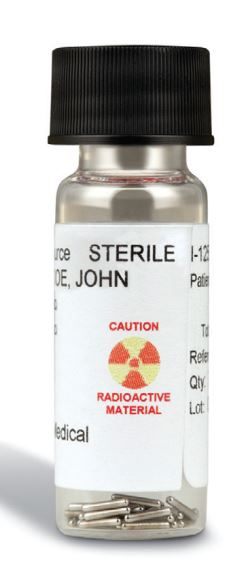
\includegraphics[width=0.10\textwidth]{Imagens/semenstesSoltasAssay.JPG}
		}%
		\caption{Sementes soltas e estéreis em frasco para ensaios.}
		\label{fig:semenstesSoltasAssay}
	\end{wrapfigure}

	Nos primeiros anos do implante de semente de próstada, as fontes estavam disponíveis apenas como sementes soltas , não esterilizadas ou esterilizadas (\ref{fig:semenstesSoltasAssay}). Os designs das sementes variam entre os fornecedores, o que causa diferenças na distribuição de dose que são grandes o suficiente de modo que é necessário que estas fontes sejam modeladas com precisão no planejamento do tratamento, mas não tão grandes que afetem a decisão sobre qual semente comprar.

	\begin{figure}[h]
		\centering
		\fcolorbox{DarkTurquoise}{white}{%
			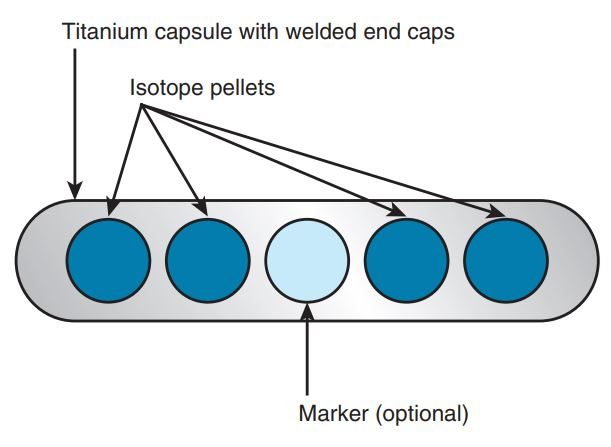
\includegraphics[width=0.35\textwidth]{Imagens/esquemaSementeProstata.JPG}
		}%
		\caption{Esquema genérico de uma semente de próstata.}
		\label{fig:esquemaSementeProstata}
	\end{figure}

	\begin{figure}[h]
		\centering
		\fcolorbox{DarkTurquoise}{white}{%
			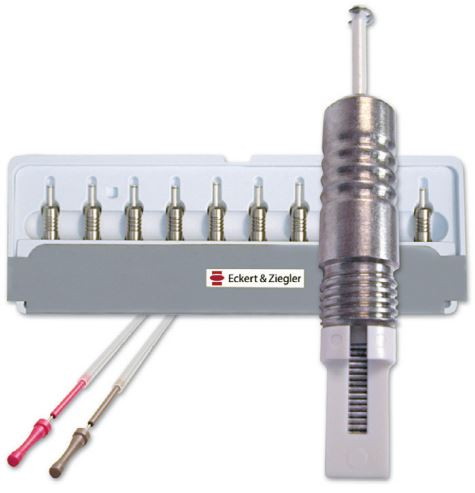
\includegraphics[width=0.35\textwidth]{Imagens/sementesSoltasMick.JPG}
		}%
		\caption{Sementes soltas no cartucho Mick.}
		\label{fig:sementesSoltasMick}
	\end{figure}

	O AAPM TG-43-U1, \textit{``A Revised AAPM Protocol for Brachytherapy Dose Calculations''}, contém desenhos detalhados para vários modelos de sementes. O esquema geral da semente é mostrado na \ref{fig:esquemaSementeProstata}. O material radioativo é acondicionado dentro de uma cápsula de titânio com tampas soldadas nas extremidades; o formato da tampa de fechamento e a textura da superfície externa podem variar. O isótopo é colocado em um substrato portador de fonte ativa e embalado em pellets (pastilhas), hastes ou cilindros. A maioria das cápsulas também contém um material de alta densidade eletrônica, como chumbo, prata, ouro ou tungstênio, como marcadores para melhorar a visibilidade das sementes nas imagens de raios-x.

	As Sementes soltas fornecem melhor flexibilidade na concepção de um implante. Os dispositivos especializados (como por exemplo, o aplicador Mick, \ref{fig:sementesSoltasMick}) estão disponíveis para automatizar o processo de carregamento de sementes soltas nas agulhas do aplicador e para reduzir a exposição da equipe. No entanto, as sementes soltas podem se migrar mais facilmente ao longo do caminho no comprimento da agulha e podem ser perdidas na bexiga ou, mais raramente, embolizar no pulmão ou mesmo no cérebro.

	
	\begin{wrapfigure}{r}{0.4\textwidth}
		\centering
		\fcolorbox{DarkTurquoise}{white}{%
			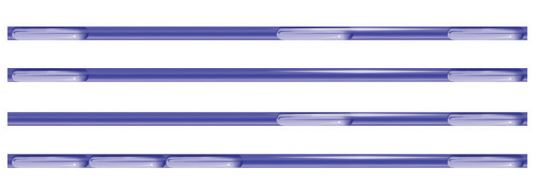
\includegraphics[width=0.35\textwidth]{Imagens/sementesAfixadas.JPG}
		}%
		\caption{Sementes fixadas em fios incluindo diferentes espaçadores.}
		\label{fig:sementesAfixadas}
	\end{wrapfigure}

	Diferentes texturas e formas foram desenvolvidas para evitar a migração de sementes. Com o tempo, as sementes em forma de fio tornaram-se disponíveis em diferentes configurações: fios/tranças de 10 fios com cadeias de até 70 sementes, agulhas pré-carregadas e dispositivos para produzir sementes fixas em forma de fios personalizados na sala de cirurgia. O material utilizado para a produção dos fios ou tranças é um material de sutura bioabsorvível. Mais recentemente, fios ecogênicos foram desenvolvidos para aumentar a visibilidade da colocação do fio com sementes durante o implante (\ref{fig:ultrassonSagitalProstataImplante}). Esses fios consistem em fios trançados de material bioabsorvível, aumentando assim a complexidade da superfície, o que melhora a visibilidade na ultrassom (US).

	\begin{figure}[h]
		\centering
		\fcolorbox{DarkTurquoise}{white}{%
			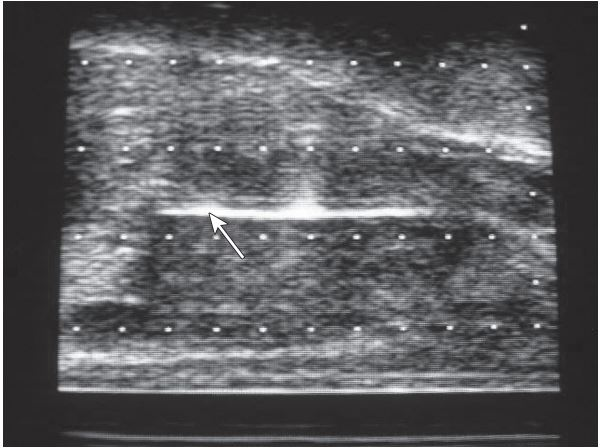
\includegraphics[width=0.5\textwidth]{Imagens/ultrassonSagitalProstataImplante.JPG}
		}%
		\caption{Imagem de ultrassom sagital de um fio ecogênico com sementes}
		\label{fig:ultrassonSagitalProstataImplante}
	\end{figure}

	A \ref{fig:sementesAfixadas} mostra um exemplo de sementes fixadas em fios. Cada sistema tem vantagens e desvantagens dependendo da tecnologia e da técnica de implante utilizada. Por exemplo, agulhas pré-carregadas requerem um pré-plano; isso resulta em eficiência na ordem das fontes porque o número exato de fontes com uma pequena margem adicional das sementes necessárias para um paciente são ordenados em comparação com a criação de uma estimativa de fonte usando um nomograma. Deve-se notar que esses nomogramas são modelos iniciais e potencialmente específicos da instituição. Por outro lado, com fios com fontes pré-ordenadas há uma inflexibilidade em ajustar o plano quando está presente na sala de cirurgia. Esses ajustes podem ser necessários nas seguintes situações:

	\begin{itemize}[label=\textcolor{CarnationPink}{$\blacktriangleright$}]
		\item Interferência do arco púbico não detectada anteriormente com a colocação de agulhas laterais anteriores;
		\item Mudança no tamanho da glândula entre o estudo do planejamento inicial e a data real do implante;
		\item Uma mudança no posicionamento (por exemplo, entre a ressonância magnética pré-planejamento e a imagem de ultrassom transretal  durante o implante) faz com que a posição da uretra e a região de avoidance retal mudem;
	\end{itemize}

	A \ref{fig:sistemasSementes} resume a utilização, as vantagens e as desvantagens dos sistemas de sementes atualmente disponíveis.

	\begin{figure}[h]
		\centering
		\fcolorbox{DarkTurquoise}{white}{%
			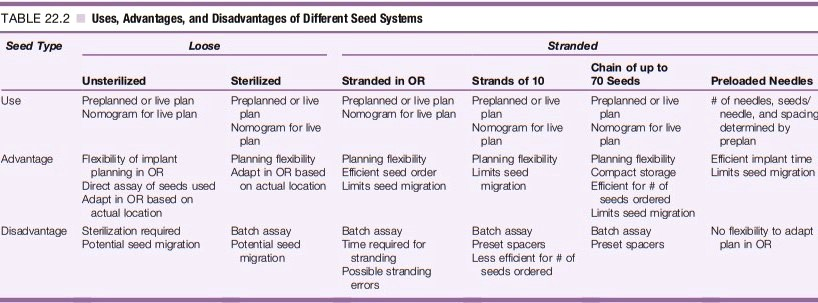
\includegraphics[width=0.95\textwidth]{Imagens/sistemasSementes.JPG}
		}%
		\caption{Características de cada semente.}
		\label{fig:sistemasSementes}
	\end{figure}

\subsection*{Ensaio de Sementes}  

	O AAPM TG-40, AAPM TG-56, \textbf{``Code of Practice for Brachytherapy Physics''}, e o AAPM TG-64, todos contêm recomendações sobre calibrações de fontes de sementes de próstata e as responsabilidades do físico médico. Esses TGs foram publicados antes que os ensaios de fontes independentes por terceiros se tornassem disponíveis. Na época, as fontes estéreis pré-montadas não estavam em uso; E também os serviços de análise independentes por terceiros ainda não estavam disponíveis. Para atualizar e esclarecer as recomendações com respeito aos ensaios, foi formado o Grupo de Trabalho de Calibração de Fontes de Braquiterapia de Baixa Energia (LEBSC WG -  \textit{Low Energy Brachytherapy Source Calibration Working Group}) pela AAPM. O white paper sobre calibrações de fontes de braquiterapia por terceiros e as responsabilidades dos físicos médicos publicado por este grupo de trabalho contém as recomendações atualizadas para as configurações de fontes atualmente disponíveis e substitui as recomendações feitas pelos TGs anteriores (\ref{fig:recomendacoesAssay}).

	\begin{figure}[h]
		\centering
		\fcolorbox{DarkTurquoise}{white}{%
			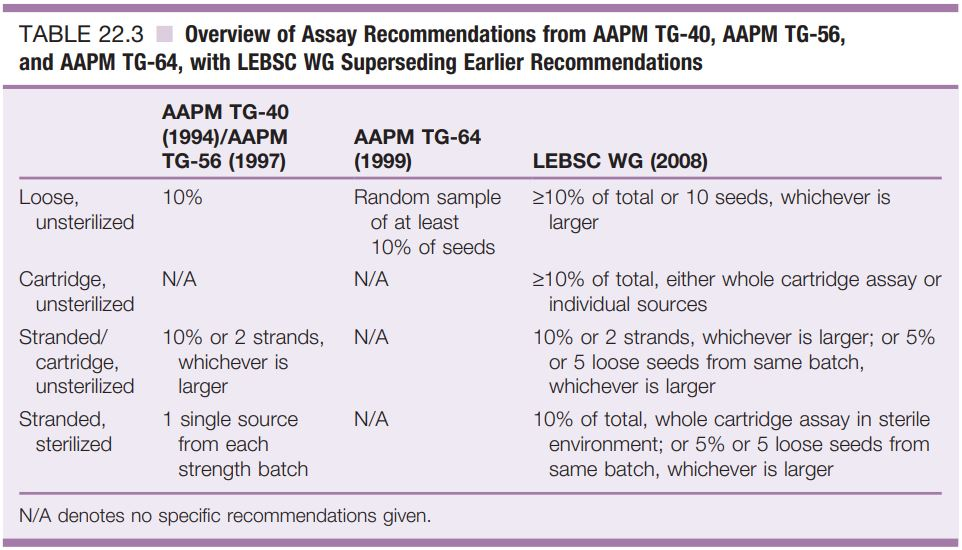
\includegraphics[width=0.8\textwidth]{Imagens/recomendacoesAssay.JPG}
		}%
		\caption{Visão geral das recomendações de ensaio das fontes dos TGs.}
		\label{fig:recomendacoesAssay}
	\end{figure}

	Depois que um fornecedor fabrica as sementes, os serviços de análise por terceiros possuem os recursos técnicos para analisar todas as sementes de um pedido e, em seguida, montá-las no pedido do cliente como agulhas ou fios pré-carregados. O usuário recebe um relatório do ensaio, contendo informações  sobre a distribuição da intensidade da semente do pedido. O padrão 170325 da International Standards Organization/International Electrotechnical Commission (ISO/IEC) fornece os requisitos para laboratórios de teste e calibração; o credenciamento sob este padrão pode servir como um indicador para a qualidade do fornecedor terceirizado que realiza o ensaio. 

	Como apontam os autores do AAPM LEBSC WG, ainda há um risco residual de erros cometidos pelo fornecedor terceirizado do ensaio. Um exemplo é o evento número 54 no report da IAEA sobre exposições acidentais em radioterapia, onde uma incompatibilidade nas unidades especificadas no pedido versus a entregue pelo fornecedor foi alcançada pelo paciente porque o ensaio do fornecedor não passou por um duplo check. Portanto, é responsabilidade do físico médico da radioterapia verificar o ensaio. Os ensaios das sementes são realizados pelo menos um dia antes do procedimento de implante para ter tempo suficiente para responder aos resultados do teste que podem estar fora da tolerância recomendada. A \ref{fig:niveisAcaoAssay} resume os níveis de tolerância fornecidos pelo AAPM LEBSC WG.

	\begin{figure}[h]
		\centering
		\fcolorbox{DarkTurquoise}{white}{%
			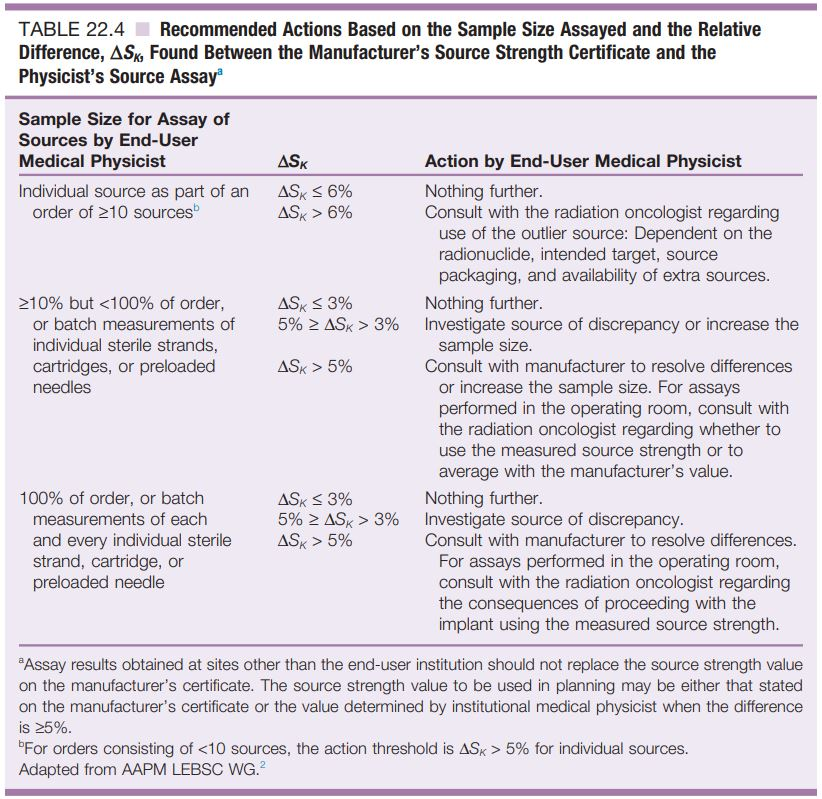
\includegraphics[width=0.6\textwidth]{Imagens/niveisAcaoAssay.JPG}
		}%
		\caption{Níveis de tolerância para os ensaios das sementes.}
		\label{fig:niveisAcaoAssay}
	\end{figure}

	
\section{Planejamento de Tratamento}

\subsection*{Planejamento Pré-Implante}

	O planejamento pré-implante pode ocorrer várias semanas ou dias antes do implante ou  então pode ocorrer na sala de cirurgia no dia do implante (também chamado de “planejamento em tempo real”). A ABS recomenda a utilização de uma ultrassom transretal (ultrassom transretal) para o planejamento pré-implante. Os implantes realizados antes de 1990 dependiam do sistema Quimby, que calcula as taxas de exposição para padrões de matriz de implantes regulares de fontes lineares e com atividades uniformes. Nessa técnica, o espaçamento entre as fontes era de 1 cm ou 2 cm. 

	Métodos de cálculo de dose e de planejamento de tratamento mais modernos levaram a uma técnica que usa um carregamento periférico das agulhas uma quantidade de agulhas internas limitadas. Esta técnica periférica modificada permitiu uma redução na dose recebida pela uretra.

\subsection*{Aquisição de Imagem Para o Tratamento}

	As imagens de ultrassom transretal, MRI ou CT podem ser usadas para o planejamento do tratamento. A imagem da TC está sendo gradualmente eliminada à medida que a RM, com seu melhor contraste de tecidos moles, está se tornando mais disponível na prática clínica (não no Brasil hehehe). Como o próprio implante será, na maioria dos casos, realizado sob a orientação da ultrassom transretal, o formato da próstata no momento do implante ficará um pouco deformado devido à presença da sonda da ultrassom transretal. Portanto, o conjunto de imagens de planejamento deve ser o mais parecido com a forma e a posição da próstata durante o implante (ou seja, ultrassom transretal na maioria dos casos). Outros estudos de imagem, como ressonância magnética, podem ser fundidos ao conjunto de imagens de planejamento. As ressonâncias magnéticas da próstata podem ser feitas usando uma bobina corporal colocada sobre a área pélvica do paciente ou usando uma bobina endorretal. Embora a bobina endorretal deforme a próstata, a anatomia resultante pode estar próxima da anatomia do implante sob a imagem da ultrassom transretal, dependendo do diâmetro e posicionamento da bobina. O médico e o físico médico devem avaliar a incerteza do registro deformável usado para fusão das imagens para escolher as margens apropriadas para os delineamentos.

	Um componente importante no estudo da imagem pré-planejamentos é avaliar a possível interferência do arco púbico. Um arco púbico estreito combinado com uma glândula relativamente grande pode tornar difícil ou impossível obter um bom acesso da agulha aos setores ântero-laterais da próstata. Pacientes com esta anatomia específica não são bons candidatos para implante de semente de próstata.

	Se uma técnica de pré-planejamento for usada, o posicionamento do paciente e da sonda da ultrassom transretal devem ser reproduzidos durante o implante porque a posição da perna e a posição da sonda afetarão muito a anatomia. Outra questão é a identificação da uretra, caso não seja utilizada um cateter de Foley. Algumas instituições injetam uma solução de gel de lidocaína aerada na uretra para torná-la visível na ultrassom transretal. Deve-se tomar cuidado para evitar gás retal e além disso a limpeza retal é frequentemente realizada antes da aquisição da imagem e do implante. É necessário um bom contato entre a sonda e a parede retal para obter uma boa imagem da próstata. Muitas vezes, um gel é injetado na tampa da sonda para ajudar a melhorar esse contato. Outros sistemas usam uma tampa de sonda sólida ou preenchida com solução salina.
	
	Um dos aspectos mais difíceis da imagem de ultrassom transretal é a identificação dos limites da próstata, principalmente a base (inferior) e o ápice (superior). Se for usado um cateter de Foley, ele pode ajudar a identificar a base da glândula por meio da visualização do balão de Foley. É comum identificar a base e o ápice e determinar o número de cortes axiais que contém a próstata. O comprimento é então confirmado em cortes sagitais.

	As instituições que usam apenas o planejamento em tempo real usarão o volume e as dimensões da próstata obtidos no pré-implante para estimar a quantidade e a força das sementes a serem solicitadas para o implante. Um nomograma é o método mais comumente utilizado para derivar esses dados. Um nomograma é definido por Merriam-Webster como “uma representação gráfica que consiste em várias linhas marcadas em escala e organizadas de tal maneira que, usando uma linha reta para conectar valores conhecidos em duas linhas, um valor desconhecido pode ser lido no ponto de interseção com outra linha”. Para um implante de semente de próstata, o nomograma é um gráfico bidimensional que relaciona o volume da próstata para uma determinada força de semente e a dose prescrita para determinar o número estimado de sementes necessárias para o implante. A \ref{fig:nomogramaImplanteProstata} mostra um exemplo de nomograma desenvolvido para implantes de sementes de próstata para determinar a atividade total de sementes de \ce{^{125}I} necessárias para fornecer 145 Gy a D90 em função do diâmetro $d$ da próstata.

	\begin{figure}[h]
		\centering
		\fcolorbox{DarkTurquoise}{white}{%
			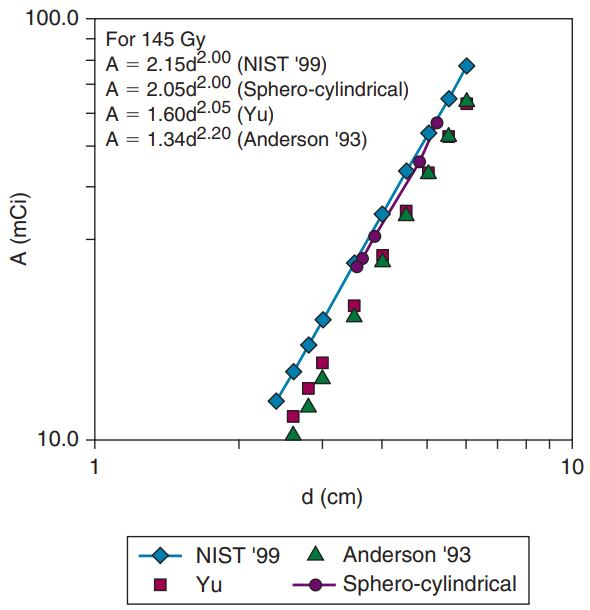
\includegraphics[width=0.8\textwidth]{Imagens/nomogramaImplanteProstata.JPG}
		}%
		\caption{Exemplo de nomograma desenvolvido para implante de semente de próstata.}
		\label{fig:nomogramaImplanteProstata}
	\end{figure}


\subsection*{Prescrição de Dose, DVH e Constraints}

	Devido às diferenças na meia-vida, as doses fornecidas pelos isótopos usados para implante de semente de próstada não podem ser comparadas diretamente. Publicações e protocolos recomendam doses diferentes para cada isótopo ou calculam BEDs (doses biologicamente efetivas) usando uma razão $\alpha/\beta$ de 2. A \ref{fig:constraintProstata} mostra vários constraints de histograma de dose-volume (DVH) de algumas selecionadas publicações, mas as doses típicas para braquiterapia como terapia exclusiva é de 145 Gy com \ce{^{125}I} e 125 Gy com \ce{^{103}Pd}; e as doses típicas para boosts de braquiterapia após teleterapia é de 110 Gy com \ce{^{125}I} e 90 a 100 Gy com \ce{^{103}Pd}.

	\begin{figure}[h]
		\centering
		\fcolorbox{DarkTurquoise}{white}{%
			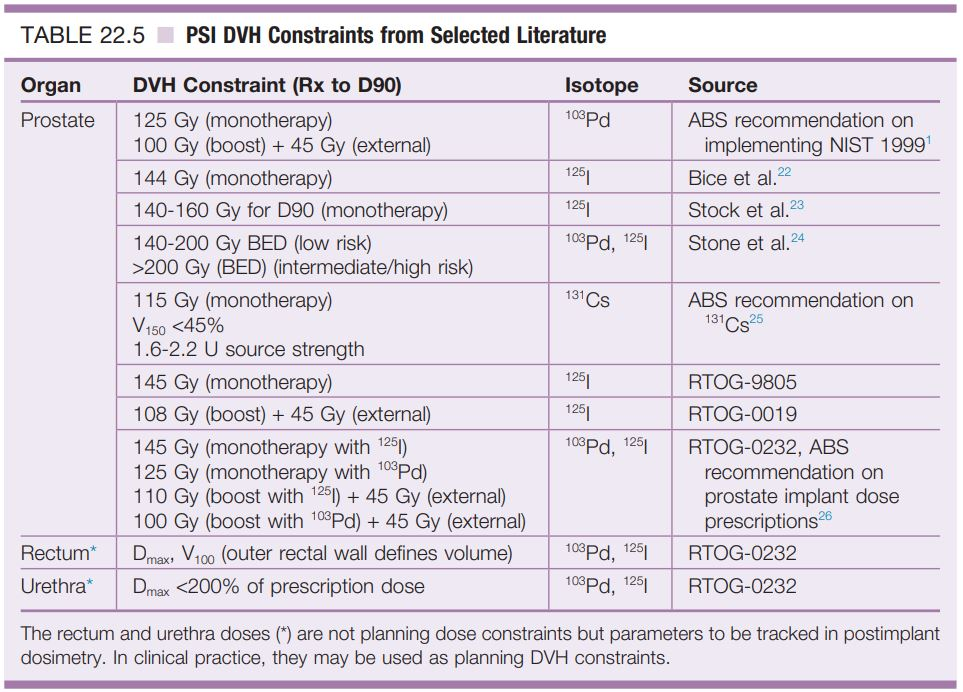
\includegraphics[width=0.8\textwidth]{Imagens/constraintProstata.JPG}
		}%
		\caption{Constraints de dose para implante de semente de próstada.}
		\label{fig:constraintProstata}
	\end{figure}

\subsection*{Diretiva Escrita}

	A NCR (10 CFR 35) regula o uso de subprodutos. A 10 CFR 35.40 abrange os requisitos e o conteúdo da diretiva escrita usada para o tratamento do paciente. A diretiva escrita tem dois componentes, \textcolor{MediumOrchid}{$(i)$} a componente antes do implante e \textcolor{MediumOrchid}{$(ii)$} a componente após o implante para permitir possíveis mudanças na estratégia do implante devido a circunstâncias médicas imprevistas que podem surgir durante o procedimento de implante. A \ref{fig:prescricaoErscrita} mostra um exemplo de diretiva escrita cumprindo os requisitos formais 10 CFR 35 Parte 40 para um implante de semente de próstata permanente usando sementes \ce{^{125}I}.

	\begin{figure}[h]
		\centering
		\fcolorbox{DarkTurquoise}{white}{%
			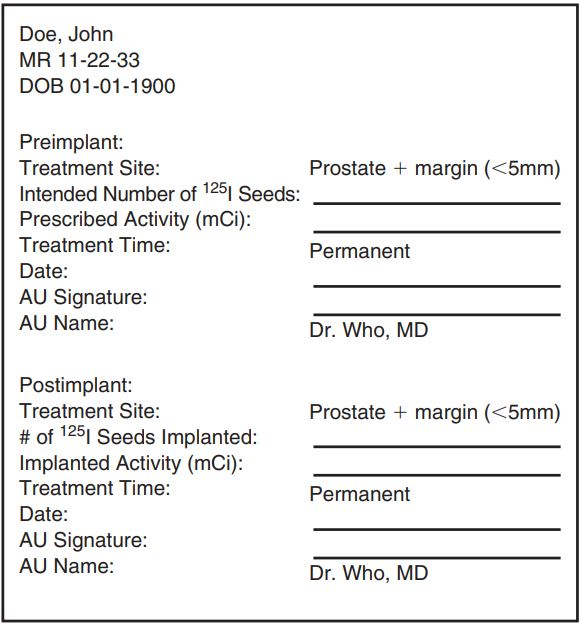
\includegraphics[width=0.8\textwidth]{Imagens/prescricaoErscrita.JPG}
		}%
		\caption{Exemplo de Diretiva Escrita.}
		\label{fig:prescricaoErscrita}
	\end{figure}

	A NRC não forneceu orientação específica sobre o que constitui a conclusão de um procedimento implante de semente de próstada na perspectiva de concluir a diretiva escrita. Recomenda-se, portanto, que cada instituição defina claramente o final do procedimento em seu protocolo de Políticas e Procedimentos (P\&P). Os pontos temporais comumente usados são \textcolor{MediumOrchid}{$(i)$} o paciente saindo da sala de cirurgia ou \textcolor{MediumOrchid}{$(ii)$} o paciente sendo liberado da recuperação. O que constitui uma conclusão precisa da diretiva escrita é um tanto controverso. No passado era utilizada uma definição baseada em dosimetria, como a dose recebida por 90\% do alvo (D90) $>$ 75\% da dose prescrita. Mais recentemente, uma definição baseada em atividade implantada foi adotada.
	
\section{Procedimento na Sala de Tratamento/Cirurgia (OR)}

\subsection*{Inserção das Agulhas}

	A inserção da agulha ocorre de forma guiada por imagem para garantir que as agulhas sejam implantadas até o plano base da próstata, mas não além, para evitar a perfuração da bexiga. A uretra e a ``bexiga bulbar''\footnote{A região da bexiga bulbar é uma parte específica da bexiga urinária localizada perto da próstata. É conhecida como "bexiga bulbar" devido à sua forma arredondada e à proximidade com a base da próstata, onde a uretra se conecta à bexiga.} são frequentemente visualizadas usando um cateter de Foley preenchido com contraste.

	É utilizada uma unidade de passo (stepper)/estabilizador (stabilizer) conectada à mesa cirúrgica para fixar/segurar a sonda da ultrassom transretal e a grade do implante (Figura 22.6). O stepper permite que a sonda da ultrassom transretal seja posicionada nas três dimensões de translação e e na rotação pitch para alinhar a sonda com o paciente. A grade do implante usada para orientação das agulhas é montada no stepper em uma posição fixa formando um ângulo reto em relação ao ultrassom transretal. No comissionamento e durante o controle de qualidade periódico, a posição da grade é calibrada em relação à sonda ultrassom transretal e ao display eletrônico da grade do implante no visor das imagens ultrassom transretal. O Teste 7 do AAPM TG-128 descreve como realizar esta calibração.

	A inserção da agulha guiada por tomografia computadorizada (TC) aumenta a dose recebida pelo paciente e pela equipe devido a imagem quando comparada ao ultrassom transretal; o baixo contraste dos tecidos moles também é outra desvantagem da TC. O implante de agulha guiado por ressonância magnética (MRI) otimiza o contraste dos tecidos moles, mas está disponível em poucas clínicas e requer um  equipamento compatível com RM. Assim, a tecnologia predominantemente utilizada para orientação por imagem durante o procedimento de implante de semente de próstada é a ultrassom transretal. A sonda da ultrassom transretal deve ter arranjos de detectores biplanares para fornecer uma imagem sagital e transversal. A próstata deve estar centralizada na grade do implante. A sonda da ultrassom transretal deve ser inclinada de forma que a borda posterior da próstata fique paralela ao trajeto da agulha. É importante ajustar a posição ântero-posterior da sonda de forma que haja um bom contato para a ultrassom, mas a pressão na próstata não deve ser tão alta a ponto de criar uma forma convexa da borda posterior da próstata. Ao usar um pré-plano, deve-se tomar muito cuidado para posicionar o ultrassom transretal o mais próximo possível da posição do pré-plano. Isso é obtido combinando a anatomia o mais próximo possível do pré-plano; a curvatura da uretra no plano sagital e as calcificações na glândula são bons pontos de referência.

	A ordem de colocação das agulhas depende da preferência do médico, que pode ser uma colocação individual, uma colocação por fileira, localizações periféricas e centrais ou todas de uma vez. Um braço-C portátil é frequentemente utilizado como um dispositivo de imagem auxiliar para a ultrassom transretal para ajudar na visualização das agulhas. A próstata incha devido ao edema causado pelo posicionamento das agulhas e também pode mudar de posição em relação ao local onde a agulha fixa uma parte da anatomia, o que pode causar incertezas de localização para algumas técnicas de implante. Uma técnica que pode corrig
	ir de forma confiável a anatomia da próstata é a seguinte:

	\begin{enumerate}[label=\textcolor{CarnationPink}{\arabic*${}^\circ$}]
		\item Colocação de duas agulhas centrais à esquerda e à direita da uretra para fixar o centro da glândula.
		\item Montar as fileiras de implantes das fileiras anteriores às posteriores; isso tem a vantagem de que eventual interferência do arco púbico seja detectada no início do implante, onde os ajustes no plano ou no implante são mais fáceis.
		\item Dentro de cada fileira, o implante de agulha deve ser feito de forma alternada começando na linha média e movendo-se para fora, alternando os lados.
	\end{enumerate}

\subsection*{Manuseio e Monitoramento das Sementes}

	No dia do procedimento, um físico autorizado removerá as fontes da sala de armazenamento das fontes e as transportará nos recipientes de proteção apropriados para a sala de cirurgia. As fontes devem estar sempre sob supervisão pessoal de um usuário autorizado. Como parte do equipamento, o usuário autorizado deve ter uma pinça, um monitor de área, e um recipiente/container adicional, ambos prontamente disponíveis para recuperar sementes que possam cair acidentalmente durante o procedimento. Imediatamente após o procedimento, uma contagem de sementes deve ser realizada para contabilizar todas as sementes radioativas.

		Os seguintes levantamentos radiométricos devem ser realizados e documentados durante o procedimento:

		\begin{enumerate}[label=\textcolor{CarnationPink}{\arabic*${}^\circ$}]
			\item Monitoramento da sala de cirurgia antes da chegada do paciente para estabelecer níveis de radiação de fundo;
			\item Monitoramento do paciente antes do início do procedimento para estabelecer o bg do paciente;
			\item Monitoramento das lixeiras, bolsa de cistoscopia, mesas de instrumentos e piso da sala de cirurgia;
			\item Monitoramento do paciente para determinar se os critérios para liberação do paciente foram atendidos.
		\end{enumerate}

\subsection*{Análise do Plano e Imagem de Acompanhamento Pós-Implante}

	Os guidelines da ACR-ASTRO para a braquiterapia de implantes transperineal permanentes par tratamento do câncer de próstata afirma que a dosimetria pós-implante é um componente obrigatório do implante de semente de próstada para todos os pacientes, e os estudos indicam que a adesão a esta determinação isso é muito alta. O objetivo do monitoramento pós-implante é verificar a contagem de sementes, o local de inserção das sementes e a dosimetria. As recomendações da ABS para análise dosimétrica pós-implante de braquiterapia permanente são um recurso para a elaboração de guidelines quanto a dosimetria pós-implante na prática clínica. 

	Semelhante à teleterapia, o implante de semente de próstada apresenta incertezas técnicas e dosimétricas que devem ser avaliadas. No feixe externo, isso é obtido usando um QA de rotina, bem como estudos de incertezas do tipo A e do tipo B (erros aleatórios e sistemáticos) durante o tratamento do paciente. Como o implante de semente de próstada é um tratamento com fração única, o desafio está em avaliar a dose total entregue durante a vida útil do implante. A migração das sementes (limitada com o uso de sementes fixadas em fios/fitas) e o edema são os fatores dominantes que introduzem incertezas ao implante de semente de próstada.

	A dosimetria pós-implante serve para avaliar a qualidade do implante e a cobertura dosimétrica do alvo, fornecendo uma métrica de controle de qualidade contínua e dá ao médico a oportunidade de antecipar possíveis complicações ou implantar sementes/complementos adicionais de dose com irradiação com feixes externos caso forem identificadas áreas de subdosagem significativas. Isso é particularmente importante, uma vez que o valor D90 pós-implante demonstrou estar correlacionado com a sobrevida livre de progressão da doença. 

	O momento da dosimetria pós-implante varia entre as instituições, desde uma imagem de verificação pós-implante no mesmo dia até uma imagem cerca de 30 dias após o procedimento. Não há dados clínicos sobre o tempo ideal para acompanhamento. O edema e o sangramento fazem com que a glândula inche durante o procedimento; a meia-vida média de resolução do edema é de cerca de 10 dias, porém com grandes variações entre os pacientes. A dosimetria pós-implante realizada imediatamente após o procedimento (ultrassom transretal) ou em até 24 horas (TC) costuma ser a mais prática, além de ter a vantagem de identificar imediatamente possíveis áreas subdosadas. O inchaço da glândula fará com que a dose total de tratamento entregue seja subestimada em cerca de 10\%.

	Um monitoramento para acompanhamento realizado 30 dias após o implante fornece as informações dosimétricas mais precisas para \ce{^{125}I}; um monitoramento para acompanhamento feito com 2 semanas seria mais apropriado para \ce{^{103}Pd}, mas o erro introduzido pela realização de um acompanhamento de 30 dias é menor. Em resumo, embora o momento exato dos estudos pós-implante ainda seja um tanto controverso, os guidelines gerais estão começando a surgir. Uma pesquisa de 2010 da ABS indica que a grande maioria das práticas (73\%) realiza a dosimetria pós-implante $\mathrm{30^{\circ}}$ dia do implante.

	Embora filmes ortogonais possam ser usados para visualizar e confirmar a contagem de sementes após um procedimento de implante, o método é subótimo para dosimetria pós-implante porque não permite a avaliação do contorno do órgão e do DVH. A ultrassom transretal é comumente usada para avaliação pós-procedimento realizada imediatamente após o implante na sala de cirurgia. Os sistemas ultrassom transretal modernos, especialmente se usados em conjunto com a fluoroscopia com braço em C, permitem uma visualização suficientemente boa dos fios implantados tornando possível criar um plano de boa qualidade para avaliação da qualidade do implante dentro da sala cirúrgica. O acesso ao sistema da ultrassom transretal de fora da sala de cirurgia, a reprodutibilidade do posicionamento da ultrassom transretal e a natureza invasiva da modalidade da imagem tornam a ultrassom transretal uma técnica raramente utilizada para dosimetria pós-implante fora da sala de cirurgia.

	Nos primeiros tratamentos de próstata feitos com implantes de sementes, eram realizadas radiografias pós-implante para verificar possíveis migração de sementes no pulmão e/ou cérebro. Este procedimento foi amplamente abandonado por várias razões, sendo elas:

	\begin{itemize}[label=\textcolor{CarnationPink}{$\blacktriangleright$}]
		\item A migração das sementes para o pulmão ou para cérebro era um evento raro em implantes com sementes soltas;
		\item O aumento do uso de sementes fixadas em fios diminuiu ainda mais a probabilidade de migração das sementes;
		\item Mesmo que fosse detectado a migração de uma semente, a informação geralmente não levava a uma ação porque o risco de um procedimento invasivo para remover as sementes perdidas era muito maior do que a relativamente pequena dose de radiação de uma semente errante;
		\item O raio-x gerava uma dose desnecessária nos pulmões e no cérebro.
	\end{itemize}

	A imagens de TC e RM são adequadas para a realizar a dosimetria pós-implante, sendo ambas técnicas não invasivas e ambas permitem a reconstrução de imagens 3D para avaliação dosimétrica e avaliação do contorno. As sementes são mais difíceis de serem localizadas na RM do que na TC porque elas representam áreas “sem sinal” semelhantes as calcificações e as áreas sem sinal imediatamente fora da cápsula da glândula. O principal desafio para a dosimetria pós-implante utilizando TC é a incerteza de contorno adicionada na base e no ápice da glândula devido à falta de contraste dos tecidos moles em comparação com outras modalidades de imagem. A fusão de imagem multimodal pode fornecer uma incerteza adicional no contorno da glândula; Além disso, alterações na anatomia entre as sessões de aquisição das imagens exigirão o registro de imagem deformável, o que também introduz incerteza no contorno.

	A \ref{fig:RecomendacoesPosImplanteProstata} resume as recomendações sobre os parâmetros de relatórios pós-implante.

	\begin{figure}[h]
		\centering
		\fcolorbox{DarkTurquoise}{white}{%
			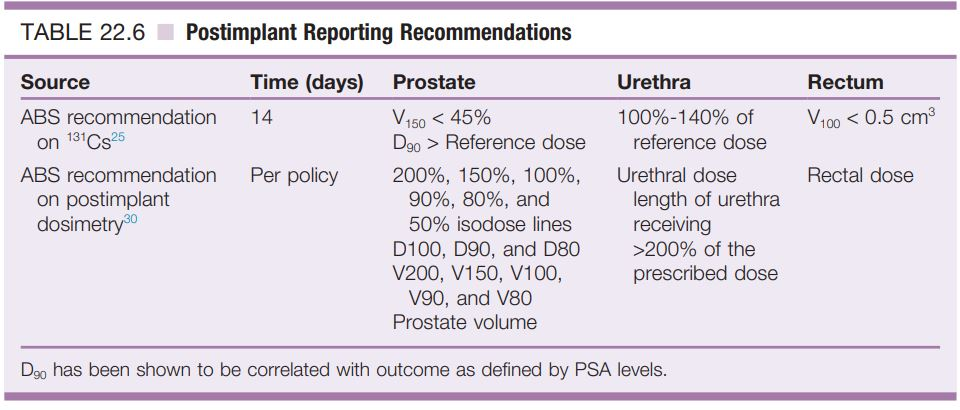
\includegraphics[width=0.8\textwidth]{Imagens/RecomendacoesPosImplanteProstata.JPG}
		}%
		\caption{Recomendações para o Report pós-implante.}
		\label{fig:RecomendacoesPosImplanteProstata}
	\end{figure}


\section{Segurança, Políticas e Procedimentos}

\subsection*{Internação e Alta do Paciente}

	De acordo com a regulação CFR 10 35, os pacientes podem ser liberados (com instruções escritas e orais) caso a dose para qualquer outro indivíduo exposto ao paciente provavelmente não exceda 5 mSv (0.5 rem). O  NUREG-1556, vol. 9, Rev. 2, \textbf{``“Program-Specific Guidance About Medical Use Licenses''} afirma que uma taxa de dose $\leq$1 mrem/h a 1 metro para pacientes com implantes de \ce{^{125}I} atende aos critérios estabelecidos pela CFR 10. Não é necessário fornecer instruções caso a taxa de dose a 1 m seja $\leq$1 mrem/h.

	Se a taxa de dose exceder 1 mrem/h, é necessário que o paciente seja internado até que a atividade da fonte diminua para um valor menor que os critérios de liberação. Devem ter estabelecidos as Políticas e procedimentos de modo que exista a sinalização da presença de radiação exigida por lei, bem como o treinamento da enfermagem e outros funcionários com respeito a exposição à radiação tanto para a equipe quanto para os visitantes. Caso uma situação especial surja, quando o paciente está cumprindo os critérios de taxa de dose para sua liberação, mas desenvolve problemas médicos durante sua recuperação que requer internação, a clínica deve desenvolver um processo para garantir que os médicos que atendam este paciente notifiquem o físico médico.

\subsection*{QA e Manutenção do Equipamento}

	O AAPM TG-128 fornece uma orientação detalhada sobre o QA para sistemas de ultrassom transretal utilizados na implante de semente de próstada. O documento técnico da  ACR para os físicos médicos quanto ao monitoramento de equipamentos de ultrassom em tempo real fornece orientação geral sobre controle de qualidade de ultrassom para a radiologia diagnóstica. O controle de qualidade do sistema de planejamento de tratamento deve seguir os conceitos gerais descritos no AAPM TG-53,\textbf{``Quality Assurance for Clinical Radiotherapy Treatment Planning''}  com cálculos de dose referentes às recomendações fornecidas pela AAPM TG-43 e suas atualizações e suplemento.

	O equipamento utilizado no implante de semente de próstada deve passar por esterilização entre os procedimentos e geralmente é armazenado longe do departamento de Radioterapia, próximo à sala de cirurgia (por exemplo, o stepper e a ultrassom transretal). É essencial treinar todos os funcionários envolvidos com respeirto ao manuseio adequado e quanto a fragilidade do equipamento. As peças que são calibradas mecanicamente (por exemplo, as anilhas que definem a posição da grade acima da ultrassom transretal) precisam ser verificadas periodicamente quanto a sua integridade e precisão. Se possível, a posição mecânica correta das peças calibradas deve ser marcada.

\subsection*{Políticas e Procedimentos}

	O implante de semente de próstada é um procedimento complexo que envolve duas especialidades médicas (Urologia e Radio-Oncologia), sala de cirurgia e enfermeiras do centro cirúrgico, físicos médicos, técnicos de sala de cirurgia e técnicos de radioterapia. Na fase de comissionamento de um novo programa de implante de sementes de próstata, é importante desenvolver orientações claras sobre as funções e responsabilidades de cada membro da equipe. Realizar uma simulação do processo de tratamento completo, desde a imagem inicial de US até o planejamento pós-implante final, é uma ferramenta útil para testar procedimentos e encontrar possíveis elos fracos ou identificar áreas onde mais esclarecimentos são necessários. Usando phantoms para implantes de sementes de próstata comerciais e sementes fictícias, as execuções de teste do procedimento de implante são bastante viáveis e fornecem oportunidades de treinamento úteis para a equipe de atendimento ao paciente.

	A \ref{fig:documentacaoPSI} mostra um exemplo de conjunto de procedimentos e documentos de orientação que são úteis para definir os padrões dos procedimentos e garantir que os requisitos regulatórios sejam obedecidos. Os procedimentos e documentos para orientação devem ser armazenados em local de fácil acesso a todos os funcionários envolvidos no programa de implante de semente de próstada. Se os documentos forem armazenados digitalmente, eles devem ser bloqueados para evitar alterações, a menos que estejam sob revisão formal. Os procedimentos e documentos para orientação devem ser revisados anualmente; quaisquer alterações devem ser comunicadas a todos os funcionários envolvidos por meio de um processo de leitura e assinatura.
	
	\begin{figure}[h]
		\centering
		\fcolorbox{DarkTurquoise}{white}{%
			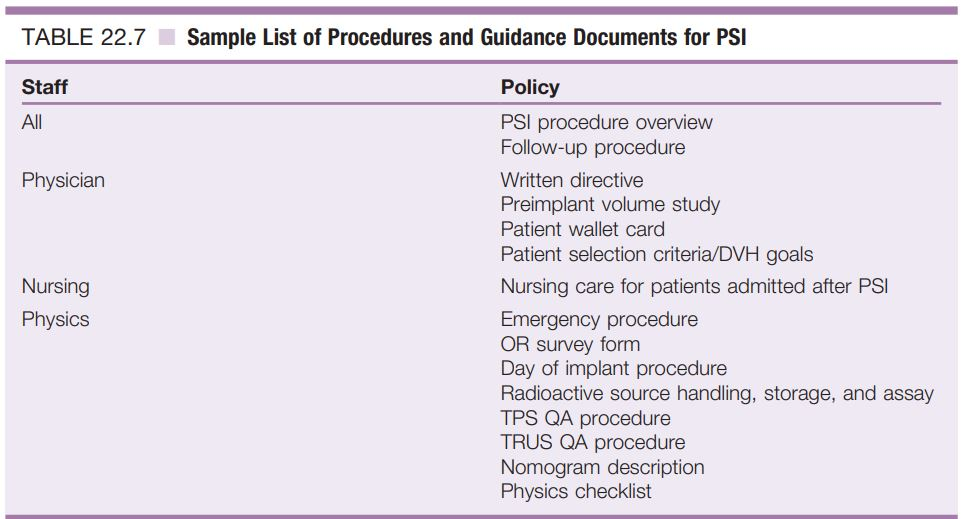
\includegraphics[width=0.8\textwidth]{Imagens/documentacaoPSI.JPG}
		}%
		\caption{Lista de Procedimentos e Documentos De Orientação para implante de semente de próstada.}
		\label{fig:documentacaoPSI}
	\end{figure}

\subsection*{Requisitos de Pessoal e Tempo}

	O tempo para cada etapa do processo pode variar de acordo com a técnica utilizada e a habilidade relativa dos membros da equipe. A \ref{fig:tempoEstiomadoImplantesStaffs} mostra um exemplo de estimativas de tempo para cada etapa de um procedimento utilizando sementes em forma de fios e com planejamento de tratamento intraoperatório, incluindo a equipe envolvida no procediumento. É útil para cada centro analisar o tempo e a equipe necessária para cada etapa do procedimento para permitir a alocação adequada de recursos.

	\begin{figure}[h]
		\centering
		\fcolorbox{DarkTurquoise}{white}{%
			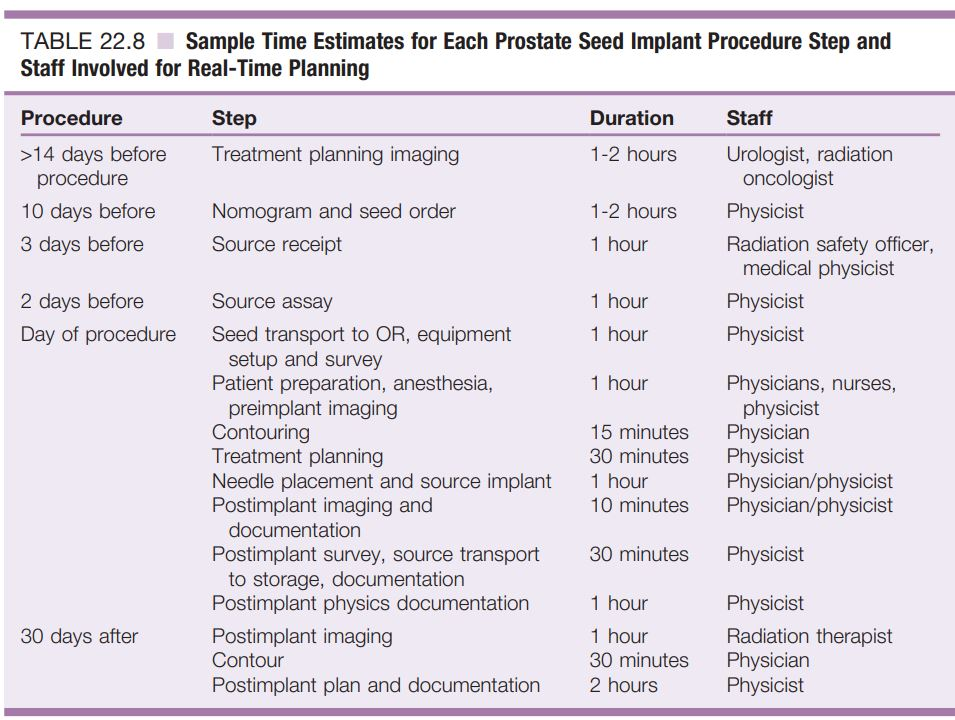
\includegraphics[width=0.8\textwidth]{Imagens/tempoEstiomadoImplantesStaffs.JPG}
		}%
		\caption{Exemplo de estimativas de tempo para cada etapa do procedimento de implante de sementes de próstata e da equipe envolvida em um caso de planejamento em tempo real.}
		\label{fig:tempoEstiomadoImplantesStaffs}
	\end{figure}


\bibliography{ref.bib}
\end{document}